\section{Appendices}

\appendix

\section{Full Object Detection Results}

Tables \ref{fig:modelsummary}, \ref{fig:aieltresults}, and \ref{fig:artresults} provide a more detailed summary of the object detection models and results on the AI-ELT and ART-Net datasets. We summarise the models, their architectures, the number of parameters, the number of layers, the main loss functions used, the inference time per image, and the FPS for each model. We also provide the mAP at 50\% and 50-95\% at 0.5 IoU threshold for the tool, tooltip, and both classes, as well as the training epochs, training time, and time per epoch for each model.

\begin{table*}[h]
\centering
\caption{Full Object Detection Models Summary.}
\label{fig:modelsummary}
\begin{tabular}{|c|c|c|c|c|c|c|c|c|}
\hline
\multicolumn{6}{|c|}{\textbf{Model Architecture}} & \multicolumn{2}{c|}{\textbf{Inference}} \\
\hline
\textbf{Model Name} & \textbf{Anchor} & \textbf{Architecture} & \textbf{Params} $^a$ & \textbf{Layers} & \textbf{Loss Function} & \textbf{Time}  $^b$ & \textbf{FPS} \\
\hline
YOLOv10-X & Anchor-based & YOLOv10 & 31.7 & \textbf{688} & YOLOv10 Loss $^c$ & 19.3 & 51.8  \\ 
YOLOv10-L & Anchor-based & YOLOv10 & 25.8 & 628 & YOLOv10 Loss & 13.0 & 76.9  \\ 
YOLOv10-B & Anchor-based & YOLOv10 & 20.5 & 518 & YOLOv10 Loss & 10.3 & 97.1  \\ 
YOLOv10-M & Anchor-based & YOLOv10 & 16.5 & 498 & YOLOv10 Loss & 8.0 & 125.0  \\ 
YOLOv10-S & Anchor-based & YOLOv10 & 8.1 & 402 & YOLOv10 Loss & 3.9 & 256.4  \\ 
YOLOv10-N & Anchor-based & YOLOv10 & 2.7 & 385 & YOLOv10 Loss & 2.2 & 465.1  \\ 
YOLOv8-X & Anchor-free & YOLOv8 & \textbf{68.2} & 385 & YOLOv8 Loss $^d$ & 21.7 & 46.1  \\ 
YOLOv8-L & Anchor-free & YOLOv8 & 43.6 & 365 & YOLOv8 Loss & 12.8 & 78.1  \\ 
YOLOv8-M & Anchor-free & YOLOv8 & 25.9 & 295 & YOLOv8 Loss & 8.0 & 125.0  \\ 
YOLOv8-S & Anchor-free & YOLOv8 & 11.1 & 225 & YOLOv8 Loss & 3.4 & 294.1  \\ 
YOLOv8-N & Anchor-free & YOLOv8 & 3.0 & 225 & YOLOv8 Loss & \textbf{1.8} & \textbf{555.6}  \\ 
RetinaNet & Anchor Non-Optimized & ResNet 50 & 36.4 & 195 & IoU + Focal Loss & 5.1 & 196.1  \\ 
RetinaNet-Opt & Anchor Optimized & ResNet 50 & 36.4 & 195 & IoU + Focal Loss & 5.2 & 192.3  \\ 
EfficientDet & Anchor-based & ImageNet & 6.6 & 552 & Focal Loss & 4.0 & 250.0  \\ 
SIMO-Resnet & Anchor-free & ResNet 50 & 23.5 & 231 & IoU + MSE $^e$ & 350.0 & 2.9  \\ 
SIMO-VGG & Anchor-free & VGG & 14.7 & 98 & IoU + MSE & 1280.0 & 0.8  \\ 
DETR & Anchor-free & ResNet 50 & 41.5 & 318 & IoU + DETR Loss & 35.9 & 27.9  \\ 
\hline
\end{tabular}
\newline
\footnotesize{$^a$ Trainable parameters in millions. $^b$ Inference time per image in milliseconds. $^c$ Box Objectness Loss + Class Objectness Loss + Detect Focal Loss + Box Offset Loss + Class Offset Loss + Detect Focal Loss Offset. $^d$ Detect Focal Loss + Verifocal Loss + Complete Intersection over Union (IoU). $^e$ Mean Squared Error.}
\end{table*}

\begin{table*}[h]
\centering
\caption{Full Object Detection Results on the AI-ELT dataset.}
\label{fig:aieltresults}
\begin{tabular}{|c|c|c|c|c|c|c|c|c|c|c|}
\hline
\multicolumn{1}{|c|}{} & \multicolumn{3}{c|}{\textbf{mAP$_{50}$}} & \multicolumn{3}{c|}{\textbf{mAP$_{50:95}$}} & \multicolumn{3}{c|}{\textbf{Training}} \\
\hline
\textbf{Model Name} & \textbf{Tool} & \textbf{Tooltip} & \textbf{Both} & \textbf{Tool} & \textbf{Tooltip} & \textbf{Both} & \textbf{Epochs} & \textbf{TT} $^a$ & \textbf{T/E} $^b$ \\ 
\hline
YOLOv10-X & 98.9 & 99.1 & 99.0 & 93.5 & 68.4 & 81.0 & 19 & 7.8 & 0.41 \\ 
YOLOv10-L & 98.9 & 98.3 & 98.6 & 89.4 & 67.0 & 78.2 & 15 & 3.5 & 0.23 \\ 
YOLOv10-B & 98.7 & 99.0 & 98.9 & 92.2 & 69.3 & 80.8 & 14 & 2.2 & 0.16 \\ 
YOLOv10-M & 98.2 & 98.7 & 98.5 & 90.5 & 69.1 & 79.8 & 14 & 1.6 & 0.11 \\ 
YOLOv10-S & 99.3 & 99.2 & 99.3 & 92.7 & 69.1 & 80.9 & 16 & 1.8 & 0.11 \\ 
YOLOv10-N & 99.1 & 99.1 & 99.1 & 93.5 & 69.9 & 81.7 & 19 & 1.9 & 0.10 \\ 
YOLOv8-X & 99.5 & \textbf{99.4} & \textbf{99.5} & \textbf{96.6} & \textbf{74.6} & \textbf{85.6} & 84 & 18.6 & 0.22 \\ 
YOLOv8-L & 99.5 & \textbf{99.4} & \textbf{99.5} & 95.2 & 73.0 & 84.1 & 36 & 1.6 & 0.05 \\ 
YOLOv8-M & 99.5 & \textbf{99.4} & \textbf{99.5} & 94.5 & 73.7 & 84.1 & 29 & 1.7 & 0.06 \\ 
YOLOv8-S & 99.5 & \textbf{99.4} & \textbf{99.5} & 96.0 & 73.9 & 85. 0& 66 & 1.0 & \textbf{0.02} \\ 
YOLOv8-N & 99.5 & \textbf{99.4} & \textbf{99.5} & 94.5 & 72.0 & 83.3 & 41 & \textbf{0.8} & \textbf{0.02} \\ 
RetinaDet & \textbf{99.9} & 98.4 & 99.2 & 89.1 & 65.3 & 77.2 & 99 & 25.7 & 0.26 \\ 
RetinaDet-Opt & \textbf{99.9} & 98.5 & 99.2 & 88.3 & 66.7 & 77.5 & 25 & 2.15 & 0.09 \\ 
EfficientDet & N/A & N/A & 48.5 & N/A & N/A & 33.7 & 162 & 4.77 & 0.03 \\ 
SIMO-Resnet & 15.6 & 12.5 & 14.1 & 13.4 & 10.9 & 12.2 & 16 & 1.30 & 0.08 \\ 
SIMO-VGG & 19.3 & 16.2 & 17.8 & 15.7 & 13.0 & 14.4 & 26 & 13.0 & 0.50 \\ 
DETR & 49.5 & 49.0 & 49.3 & 46.3 & 32.3 & 39.3 & \textbf{294} & 16.2 & 0.06 \\
\hline
\end{tabular}
\newline
\footnotesize{$^a$ Training Time (in hours). $^b$ Time per epoch (in hours).}
\end{table*}

\begin{table*}[h]
\centering
\caption{Full Object Detection Results on the ART-Net Dataset.}
\label{fig:artresults}
\begin{tabular}{|c|c|c|c|c|c|c|c|c|c|c|}
\hline
\multicolumn{1}{|c|}{} & \multicolumn{3}{c|}{\textbf{mAP$_{50:95}$}} & \multicolumn{3}{c|}{\textbf{mAP$_{50:95}$}} & \multicolumn{3}{c|}{\textbf{Training}} \\
\hline
\textbf{Model Name} & \textbf{Tool} & \textbf{Tooltip} & \textbf{Both} & \textbf{Tool} & \textbf{Tooltip} & \textbf{Both} & \textbf{Epochs} & \textbf{TT} $^a$ & \textbf{T/E} $^b$ \\ 
\hline
YOLOv10-X & 75.3 & 43.1 & 59.2 & 55.4 & 20.8 & 38.1 & 47 & 8.6 & 0.18 \\ 
YOLOv10-L & 57.3 & 29.0 & 43.2 & 35.0 & 12.2 & 23.6 & 19 & 1.2 & 0.06 \\ 
YOLOv10-B & 69.0 & 43.0 & 56.0 & 46.7 & 21.6 & 34.2 & 33 & 1.1 & 0.03 \\ 
YOLOv10-M & 69.6 & 26.9 & 48.3 & 46.4 & 11.0 & 28.7 & 28 & 0.6 & 0.02 \\ 
YOLOv10-S & 68.4 & 46.1 & 57.3 & 49.3 & 20.2 & 34.8 & 28 & 0.5 & 0.02 \\ 
YOLOv10-N & 75.3 & 53.6 & 64.5 & 57.3 & 28.6 & 43.0 & 48 & 0.7 & 0.01 \\ 
YOLOv8-X & 88.9 & 67.5 & 78.2 & 70.1 & 32.8 & 51.5 & 85 & 7.9 & 0.09 \\ 
YOLOv8-L & 90.4 & 61.9 & 76.2 & 70.0 & 28.6 & 49.3 & 62 & 1.6 & 0.03 \\ 
YOLOv8-M & 89.8 & 65.2 & 77.5 & 66.0 & 33.0 & 49.5 & 45 & 0.6 & 0.01 \\ 
YOLOv8-S & \textbf{93.8} & 76.5 & 85.2 & 75.2 & 37.1 & 56.2 & 73 & 0.5 & 0.01 \\ 
YOLOv8-N & 92.9 & \textbf{80.4} & \textbf{86.7} & \textbf{76.2} & \textbf{43.3} & \textbf{59.8} & 90 & \textbf{0.4} & \textbf{0.004} \\ 
RetinaDet & 86.9 & 66.5 & 76.7 & 57.1 & 41.4 & 49.3 & 42 & 1.5 & 0.03 \\ 
RetinaDet-Opt & 90.1 & 69.4 & 79.8 & 60.0 & \textbf{43.3} & 51.7 & 15 & 0.7 & 0.04 \\ 
EfficientDet & N/A & N/A & 57.0 & N/A & N/A & 38.7 & 40 & 0.5 & 0.01 \\ 
SIMO-Resnet & 17.4 & 10.1 & 13.8 & 16.9 & 15.1 & 16.0 & 15 & 3.6 & 0.24 \\ 
SIMO-VGG & 19.1 & 12.1 & 15.6 & 18.8 & 11.7 & 15.2 & 32 & 7.0 & 0.22 \\ 
DETR & 23.7 & 13.3 & 18.5 & 13.1 & 13.3 & 13.2 & \textbf{305} & 19.7 & 0.06 \\ 
\hline
\end{tabular}
\newline
\footnotesize{$^a$ Training Time (in hours). $^b$ Time per epoch (in hours).}
\end{table*}

\begin{figure}[htbp]
    \centering
    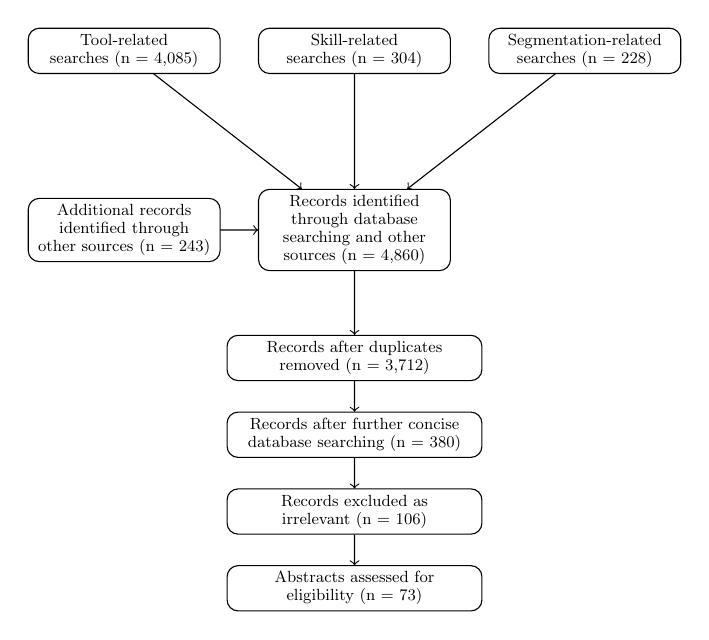
\begin{tikzpicture}[node distance=1.5cm, scale=0.65, every node/.style={transform shape, font=\fontsize{9}{10}\selectfont}]

    % Top level boxes
    \node (tool) [rectangle, draw, text width=10em, text centered, rounded corners] {Tool-related searches (n = 4,085)};
    \node (skill) [rectangle, draw, text width=10em, text centered, rounded corners, right of=tool, xshift=3cm] {Skill-related searches (n = 304)};
    \node (segmentation) [rectangle, draw, text width=10em, text centered, rounded corners, right of=skill, xshift=3cm] {Segmentation-related searches (n = 228)};

    % Box connecting to database searching
    \node (id) [rectangle, draw, text width=10em, text centered, rounded corners, below of=skill, yshift=-2cm] {Records identified through database searching and other sources (n = 4,860)};
    \draw[->] (tool) -- (id);
    \draw[->] (skill) -- (id);
    \draw[->] (segmentation) -- (id);

    % Additional records
    \node (os) [rectangle, draw, text width=10em, text centered, rounded corners, left of=id, xshift=-3cm] {Additional records identified through other sources (n = 243)};
    \draw[->] (os) -- (id);

    % Duplicates removed
    \node (dup) [rectangle, draw, text width=13.5em, text centered, rounded corners, below of=id, yshift=-1cm] {Records after duplicates removed (n = 3,712)};
    \draw[->] (id) -- (dup);

    % Screening
    \node (sc) [rectangle, draw, text width=13.5em, text centered, rounded corners, below of=dup] {Records after further concise database searching (n = 380)};
    \draw[->] (dup) -- (sc);

    % Irrelevant exclusion
    \node (ex) [rectangle, draw, text width=13.5em, text centered, rounded corners, below of=sc] {Records excluded as irrelevant (n = 106)};
    \draw[->] (sc) -- (ex);
    
    % Abstract assessed
    \node (at) [rectangle, draw, text width=13.5em, text centered, rounded corners, below of=ex] {Abstracts assessed for eligibility (n = 73)};
    \draw[->] (ex) -- (at);
    
    % % Full text assessed
    % \node (ft) [rectangle, draw, text width=13.5em, text centered, rounded corners, below of=ex] {Full-text articles assessed for eligibility (n = 73)};
    % \draw[->] (ex) -- (ft);

    % % Articles excluded after full text assessment
    % \node (fa) [rectangle, draw, text width=13.5em, text centered, rounded corners, below of=ft] {Articles excluded after full-text assessment (n = 43)};
    % \draw[->] (ft) -- (fa);

    % % Final studies included
    % \node (inc) [rectangle, draw, text width=13.5em, text centered, rounded corners, below of=fa] {Studies included in the final review (n = \textcolor{red}{XX})};
    % \draw[->] (fa) -- (inc);

    \end{tikzpicture}
    \caption{PRISMA Flow Diagram}
    \Description{The flow diagram of the paper selection and pruning process according to the recommendations of the PRISMA method.}
    \label{fig:prisma}
\end{figure}


\section{Literature Search}

This study is part of an MSc component of a PhD in Surgical Skill Improvements through AI-driven Training Enhancements. Thus, a more thorough literature search was required to inform decisions on where to begin research in this domain. The search strategy was meticulously designed to ensure a comprehensive exploration of the literature concerning surgical tool tracking and related topics. The selected databases — PubMed and Ovid - are among the most comprehensive resources for biomedical literature, ensuring that the search covers a broad spectrum of relevant research. The literature search began in April 2024, and to keep the review current, alerts were set up on PubMed to capture any newly published research. This ongoing search process, with backward and forward citation tracking and additional searches through other sources like Google Scholar, ensured the review was as comprehensive and up-to-date as possible.

Figure \ref{fig:prisma} illustrates the flow of the search, following the recommendations of the Preferred Reporting Items for Systematic Reviews and Meta-Analyses (PRISMA) statement \cite{moher_preferred_2010}. The strategy was divided into three main categories: tool-related searches, skill-related searches, and segmentation-related searches. This was not focused on conducting a systematic review but on establishing context, considering SOTA methods and models, and identifying areas for further research in AI-enhanced laparoscopic training, so no clear exclusion criteria were required. This approach allows for an understanding of the current research landscape, facilitating the identification of gaps and opportunities for this ongoing search process and future research, including the focus of this study.

\section{Object Tracking}

Our paper focuses on a simple tracking algorithm that performed excellently on our dataset. However, more advanced techniques would have to be employed to build a robust method across various other datasets. We can combine these into standard computer vision and more advanced artificial intelligence methods.

\subsubsection{Computer Vision Methods}

Many alternative tracking methods can be used for specific tasks, which can be incredibly useful with increasing accuracies of detection and tracking. Optical flow methods estimate the motion of objects between consecutive frames of video. By tracking keypoints or pixels, these methods can determine movement patterns corresponding to the tool's movement. An essential technique used in the Lucas-Kanade method utilises a different method for optical flow estimation that is efficient for small motion, which we experience in laparoscopic data. It also uses the Horn-Schunck method, which assumes smoothness in the motion field. This works well in real-time applications and can track movement across frames with moderate accuracy. We can improve the robustness and accuracy by using sensor data to initialise and help guide the optical flow tracking process. The Kalman Filter method is prevalent and widely used in tracking, which provides estimates of unknown variables by optimally combining a series of measurements observed over time, which is excellent for real-time applications and noisy data. They also offer a simple, cost-effective way to combine sensor data but are only accurate for linear motion models with Gaussian uncertainties \cite{bouget_vision-based_2017}. Despite this, they have been sufficient for many instrument detection applications. A particle filter can track the tool positions based on probabilistic models, sensor readings, and a motion model. This makes it robust to non-linearities and multi-modal distributions in the sensor data. Background subtraction is a simple method which involves separating foreground objects from the background in video frames to isolate and track moving objects. Gaussian Mixture Models can model the background using multiple normal distributions to adapt to changes in lighting, scene dynamics and camera movement. Frame differencing is the simplest method to highlight moving objects. This is extremely effective in controlled environments with static backgrounds, making it highly suitable for our application. Feature matching can track movement by detecting and matching key features such as corners and edges. With speeded-up robust features (SURF), a faster alternative to the popular scale-invariant feature transform (SIFT) method to describe local features, we can track key points in real-time applications and be robust to scale and rotation changes daily in laparoscopic videos. Template matching, where we use pre-defined templates of the tools, can locate tools and track them frame-by-frame. Its weakness is in aspect-ratio changes, which can be countered by implementing one of the aforementioned SIFT or SURF techniques. Simple edge detection and contour tracking can also be used in non-in-vivo datasets with a simpler non-moving background than in-vivo data.

\subsubsection{Artificial Intelligence Methods}

Artificial intelligence methods can be used to track tools in laparoscopic videos. We can use a deep learning method, such as a convolutional neural network (CNN), to detect image tools. Then, we can use a recurrent neural network (RNN) to use previous information to reinforce predictions in the current frame. We could also use a long short-term memory (LSTM) network to remember information over long periods or a gated recurrent unit (GRU) network, a simplified version of an LSTM network that is more efficient and can be used in real-time applications. We could use a transformer network, a deep learning model that uses attention mechanisms to learn dependencies between input and output data. Graph neural networks can model spatial and temporal relationships between objects in a scene. They can be used to track tools in a video where we consider tool positions as nodes and edges as the relationships between them. All these methods allow us to track tools in real-time applications, with the ability to learn from previous frames and predict future frames more robustly and accurately than traditional computer vision methods.

\section{Online Resources}

Other resources, including models and datasets, can be found at the following links:

\begin{itemize}[noitemsep, left=0pt]
\item \textbf{Anchor Optimisation:} \url{https://github.com/martinzlocha/anchor-optimization}
\item \textbf{Augmented Reality Tool Network (ART-Net):} \url{https://github.com/kamruleee51/ART-Net}
\item \textbf{EfficientDet:} \url{https://github.com/rwightman/efficientdet-pytorch}
\item \textbf{End-to-End Object Detection with Transformers (DETR):} \url{https://github.com/facebookresearch/detr}
\item \textbf{MICCAI 2015 EndoVis Dataset (EndoVis 2015):} \url{https://web.archive.org/web/20230323215521/https://opencas.webarchiv.kit.edu/?q=node/30}
\item \textbf{PEg TRAnsfer Workflow (PETRAW) Dataset:} \url{https://www.synapse.org/Synapse:syn25147789/wiki/608848}
\item \textbf{PyTorch RetinaNet:} \url{https://github.com/yhenon/pytorch-retinanet}
\item \textbf{Ultralytics YOLO Models:} \url{https://github.com/ultralytics/ultralytics}
\item \textbf{YOLOv10: Real-Time End-to-End Object Detection:} \url{https://github.com/THU-MIG/yolov10?tab=readme-ov-file}
\end{itemize}